\subsection{Excercise MicroArchDMCar}
%//TODO introduction
\subsubsection*{Parts of a Micro Architecture}
The microarchitecture specifies the internal code structure of the microservice.
It plays a major role in the further development and maintenance process whether on the chosen complexity.
The basic structure of a microservice's microarchitecture is divided into three separate parts: the Microservice Requester, the Microservice API, and the Persistency Interface.
Each of these parts is described in more detail in the following.

\paragraph*{Microservice Requester:}
The Microservice Requester is the software unit sending requests to the microservice and receiving the microservice's responses.
This can be the front end or another microservice.

\paragraph*{Microservice API:}
Each microservice implements and provides an API.
It is defined by the microservice's specification and is usually based on REST or gRPC depending on the microservice's requirements.
The API contains the Domain or Application logic, based on the type of microservice.
It implements the according operations and logic.
The logic is structured according to the given operations.

\paragraph*{Persistency Interface:}
This part provides the data elements like entities or value objects.
These elements can be accessed by the operations.
This enables decoupling of the interface to the database by which the data elements are stored.

\subsubsection*{Parts of the DM-CarV1.0 Micro Architecture}
The general structure of a microarchitecture has been explained in the previous section.
This task applies the general structure to the DM-CarV1.0 microservice.
The structure of the DM-CarV1.0 microarchitecture is shown in \autoref{fig:ms_dmCar_microArchitecture}.

\paragraph*{Microservice Requester:}
The DM-CarV1.0 microservice does not have a requester in this implementation.
Yet, another microservice or the front end could be the requester if the microservice is used in a real-world scenario or the microservice is extended.
Therefore the requester is not included in the graphics.

\paragraph*{Microservice API:}
The microservice API consists of the controller and the specification.
The specification is the OpenAPI specification of the microservice and describes the endpoints and operations of the microservice.
The controller implements the paths of the specification by calling the operations from the operations package.

\paragraph*{Models and Operations:}
This layer implements the domain logic of the microservice.
It contains the operations and the models.
The model package contains the entities and value objects as specified in the API diagram.
The operations package contains the operations and their according tests.
Each operation is implemented in a separate file to ensure the separation of concerns.

\paragraph*{Persistency Interface:}
The persistency interface is implemented in the \texttt{infrastructure} package.
It contains the mappers, the persistence entities, and the repositories.
The mappers provide the functions to convert \texttt{car} and \texttt{cars} model objects to persistence entities and vice versa.
The persistence entities are the entities that are stored in the database.
The repositories provide the functions to interact with the database and the in-memory repository.

\begin{figure}
    \centering
    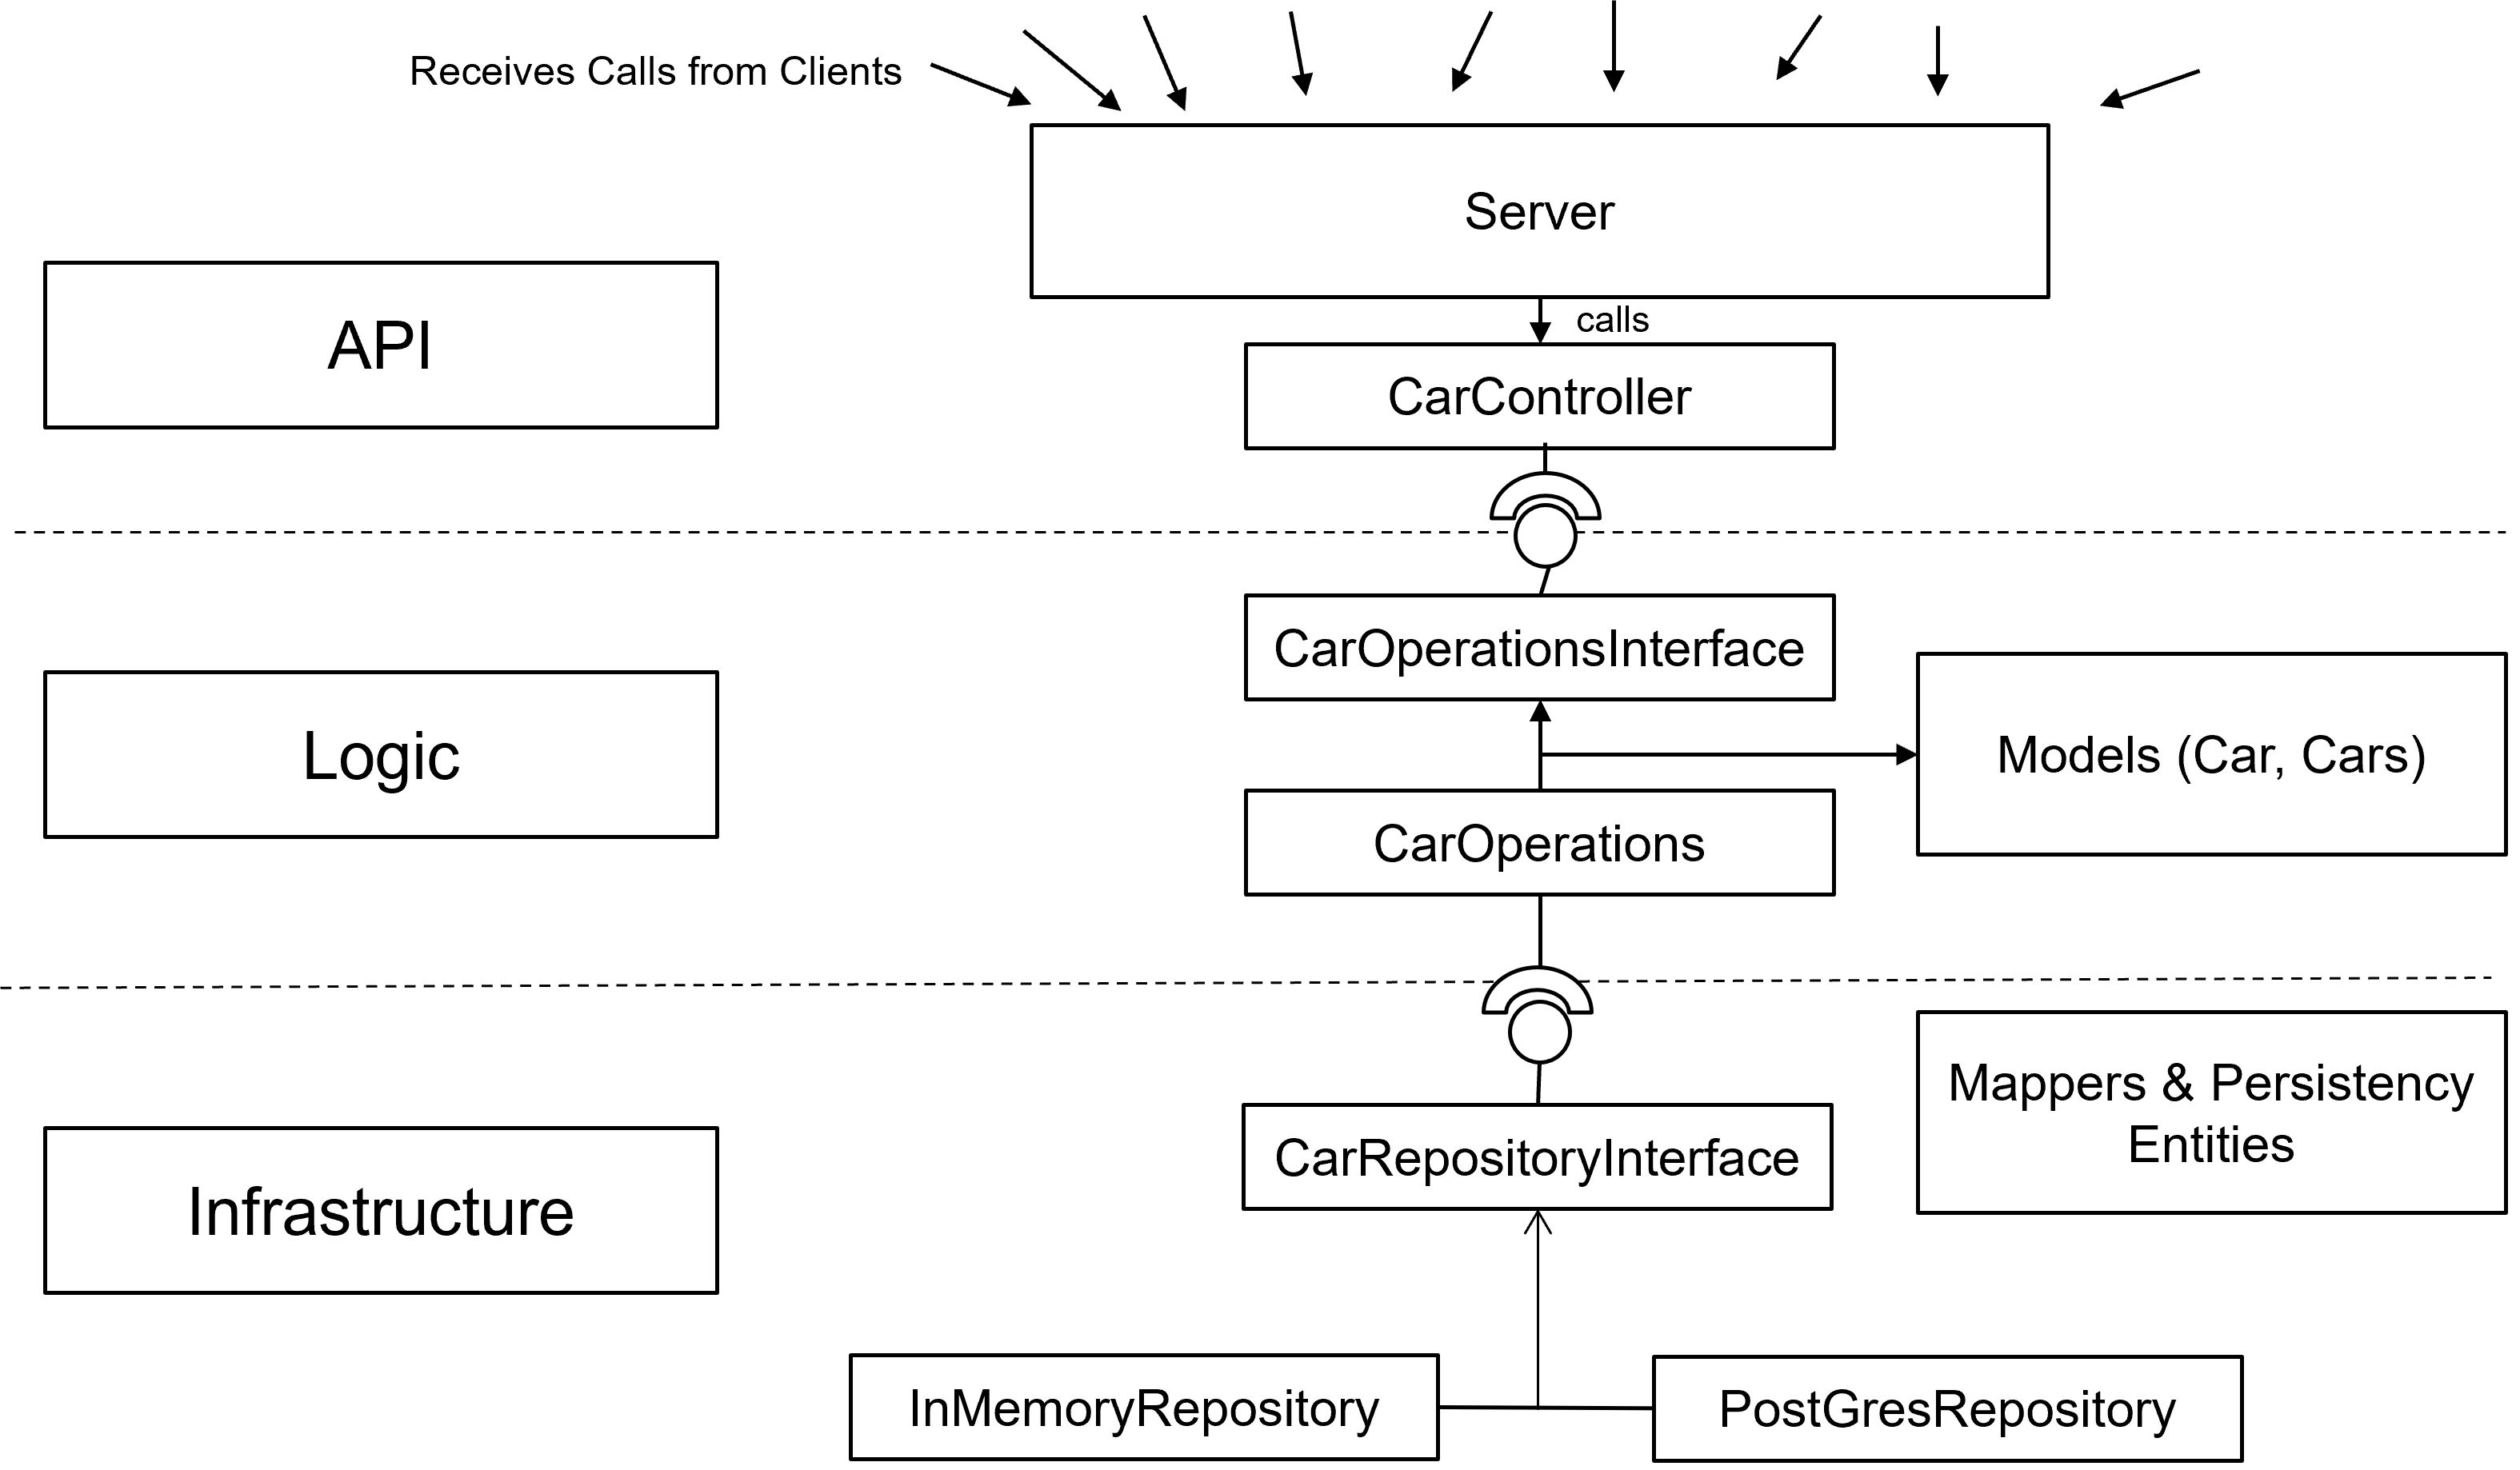
\includegraphics[width=0.8\textwidth]{figures/microservices/dmCar/ms_dmCar_microArchitecture.png}
    \caption{Micro Architecture of the DM-CarV1.0 Microservice}
    \label{fig:ms_dmCar_microArchitecture}
\end{figure}

\subsubsection*{Micro Architecture in VS Code}

\subsection{Excercise LogicPartDMCar}
\subsubsection*{Content of the Logic Folder}
\subsubsection*{Repository Interface}
\subsubsection*{Operations Interface}
\subsubsection*{Operation GetCar}


\subsection{Excercise APIPartDMCar}
\subsubsection*{Content of the API Folder}
\subsubsection*{Generated Files}
\subsubsection*{File CarController.go}
\subsubsection*{Mathod GetCar}

\subsection{Excercise InfrastructurePartDMCar}
\subsubsection*{Content of the Infrastructure Folder}
\subsubsection*{Persistence Entities}
\subsubsection*{Mappers}
\subsubsection*{InMemoryRepository}


\subsection{Excercise CSGetCar}
\subsubsection*{Code Sketch GetCar}
\subsubsection*{GetCar Flow Through the Code Sketch}


\subsection{Challenge Operation AddCar}
\subsubsection*{Update API Diagram}
\subsubsection*{Update API Specification}
\subsubsection*{Implement Operation AddCar}
\subsubsection*{Regenerate API Server}
\subsubsection*{Implement Route at API Controller}
\subsubsection*{Complete Repository Implementation}
\subsubsection*{Run Microservice}